%============================================================================%
% Author: Pablo S�nchez                                                      %
%         p.sanchez@unican.es, http://personales.unican.es/sanchezbp         %
% Section : Research Challenges                            Date: 25/02/2011  %
% Version : 1.0                                                              %
% Conference: SPLC 2011                                                      %
%============================================================================%

%============================================================================================
% NOTE(Pablo): This is not required for SPLC 2011
%============================================================================================
%
% The creation of clonable features was initially an easy task, since it only required to add
% the notion of cardinality to each feature. Nevertheless, this has created several
% side-effects, since some concepts such as the semantics of a clonable feature selection, had % to be reviewed and updated. This section identifies several problems, not currently solved to % the best of our knowledge, regarding the specification of external constraints involving
% clonable features.
%
%============================================================================================

%============================================================================================
% NOTE(Pablo): Too much verbose
%============================================================================================
%
% Nevertheless, this had several consequences, since it was required to review an update
% well-established concepts related to feature modelling and to answer several research
% challenges that emerged as a consequence of introducing this new concept. Previous section
% described how clonable features are selected by means of a new cloning operation. This
% section identifies several problems, not currently solved to the best of our knowledge,
% regarding the specification of external constraints between features when some of the
% features involved in the constraint are clonable.
%
%============================================================================================

Clonable features creates new challenges when the specification of cross-tree constraints is required. For instance, according to Figure~\ref{fig:smartHomeFM}, house facilities can be selected at a house, floor or room level. Therefore, a cross-tree constraint should specify if \imp{LightMng} has been selected at the floor level, this facility must also have been selected for each room belonging to that floor.

Since \imp{SmartEnergyMng} requires the \imp{HeaterMng} and \imp{WindowMng} features have been selected, other constraint should specify whenever \imp{SmartEnergyMng} has been selected at one level (e.g. for a specific floor), \imp{HeaterMng} and \imp{WindowMng} have also been selected at the same level (i.e. for that specific floor). Finally, we might want to specify more advanced constraints, like if \imp{Presence Simulation} is going to be included in a automated house, a 30\% of the rooms in the house at least must include automatic light management .

In feature models, the most usual way to express cross-tree constraints is using propositional logic formulas, such as \imp{SmartEnergyMng implies (LightMng and HeaterMng)}, where the different features are the atoms for these formulas~\cite{batory:2005}. An atom is evaluated to true when the corresponding feature has been selected, otherwise it is false. The main problem when dealing with clonable features is that this correspondence cannot be used. Clonable features are not selected or unselected. Clonable are just cloned. So, the meaning of a atom related to a clonable feature becomes undefined. As a result, a propositional logical formula including clonable features can not be evaluated and it can not be determined when the corresponding constraint has been satisfied or violated.

For instance, let us suppose  \imp{A} and \imp{B} are clonable features. In this case, what would be the meaning of a external constraint like \imp{A implies B}? Does this means that one instance of \imp{A} implies the existence of at least one instance of \imp{B}? Or, on the other hand, does it means that the existence of all potential \imp{A}s implies the existence of all potential \imp{B}s? Or, why not, the existence of all potential \imp{A}s implies the existence of only one \imp{B}? So, the first research challenge we face is to decide what a clonable feature exactly means in a logical formula expressing a cross-tree constraint.

Since each clonable feature really evaluates to a set of clones, we might want to specify properties that only applies to: (1) at least one element of the set; (2) to all the elements of the set that fulfill a certain constraint; or (3) all the elements of the set. For instance, we might want to specify constraint such as: if \imp{HeaterMng} is selected per house level, one \imp{Room} at least must contain one \imp{Heater} as a minimum. So, our second research challenge is to add quantification mechanisms to constraints involving clonable features.

% Por aqu�

Moreover, as already commented we might want to specify constraints which must be evaluated for a particular subtree of the whole feature model, i.e. in a particular \emph{context}. For instance, if \imp{LightMng} has been selected as facility for a particular \imp{Room}, such a \imp{Room} must have one instance of the \imp{Light} feature at least. If we specified a constraint ``\imp{LightMng} implies \imp{Light}'' at least one, but we did not limit the scope in which this constraint is evaluated, this constraint might be true for the configurations of Figure~\ref{fig:contexts} (a) and (b). Nevertheless, this constraint should be false for Figure~\ref{fig:contexts} (a), since \imp{r1:Room} has selected the \imp{LightMng} facility, but it has not \imp{Light} to control. This means this constraint must be evaluated for all rooms (notice we need again quantification) and using only the subtree below each \imp{Room}. Thus, the third research challenge is to specify the context where each constraint must be evaluated.

% Figure~\ref{fig:contexts} contains an example and a counterexample for this situation.

% i.e. we use the whole feature model for evaluating the constraint, this constraint will be true for the configuration of
% Figure~\ref{fig:contexts} (a) and (b). Nevertheless, this constraint should be not satisfied by the configuration of
% Figure~\ref{fig:contexts} (a) is not correct, since \imp{r1:Room} has selected the \imp{LightMng} facility, but it has
% not \imp{Light} to control.

% Contexts are also useful for solve ambiguities when using feature references, since multiple copies of a same feature
% might appear at different part of a configuration model. For instance, does \imp{LightMng} refers to \imp{LightMng} for
% \imp{GeneralFacilities}, \imp{FloorFacilities} or \imp{RoomFacilities}. Using contexts, we can limit the scope of a name % to unambiguously refer to a certain feature.

\begin{figure}
  % Requires \usepackage{graphicx}
  \centering 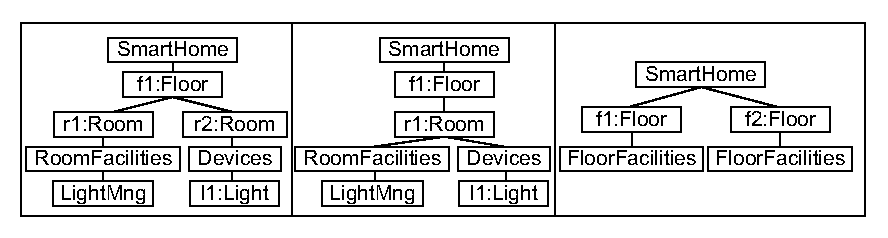
\includegraphics[width=.7\linewidth]{Figures/contexts(2).eps} \\
  \caption{(a) Invalid configuration (b) Valid configuration (c) Multiple features}
  \label{fig:contexts}
\end{figure}

Finally, when dealing with clonable feature, not only clonable features can appear more than one time in a configuration model. A feature can appear more than one time one of its ancestors is clonable. Figure~\ref{fig:contexts} (a) illustrates this situation. We call to a feature that can appear more than one time a \emph{multiple feature}. For instance, the feature \imp{FloorFacilities}, which is not clonable itself,  might appear several times in a configuration model as a consequence of the \imp{Floor} feature being cloned. This implies that \imp{FloorFacilities} also evaluates to a set of features when it is evaluated in the context of the entire configuration model. Nevertheless, it should be noticed that this feature can be evaluated to true or false if it is evaluated in the context of a \imp{Floor} feature, since it can appear only once in that context. So, a last research challenge is how to deal appropriately with \emph{multiple features}.

Summarising, when dealing with clonable features, we need to address the following research challenges in order to properly express constraints between features:

\begin{enumerate}
	\item What a clonable feature means inside a constraint expression.
	\item Add quantification mechanisms to constraints expressions.
	\item Add the notion of contexts to constraints expressions and subexpressions.
	\item Design a mechanism for properly dealing with clonable features.
\end{enumerate}

State-of-art tools only offer two operators, \imp{implies} and \imp{excludes}, and deal with simple propositional formulas. This is clearly not enough to address the research challenges described in this section.
To solve this limitation, we have created an expressive language for expressing arbitrary complex constraints in a user-friendly fashion and we have implemented a reasoner able to decide if a set of external constraints, involving
clonable or multiple features, is satisfied given a specific configuration of a feature model. The reasoner is also able to perform some extra task, such as deciding which features must be incorporated to a configuration in order to satisfy the external constraints. We have integrated this language and the reasoner in our feature modelling environment, which we have called \emph{Hydra}.

Next section describes the language for expressing external constraints involving clonable features and the reasoner that analyse the satisfiability of these constraints.

%\emph{Hydra}, a tool for modelling, configuring and validating cardinality-based features models, i.e. feature models
% that contain \emph{clonable features}. This has implied we have had to review the way in which clonable features are
% configured, and, overall, how user-defined constraints are defined and evaluated in the presence on clonable
% features.

%==================================================================================================%
% NOTE(Pablo): Out                                                                                 %
%==================================================================================================%

% A typical feature modelling process would be as follows:
%
% \begin{enumerate}
%    \item First of all, a feature model is created. A feature model is a tree representation of the features included in % a set of products and of the relationships between them.
%    \item Since not all the relationships between features can be captured using simply the syntax provided by feature
% models, it is often required to specify some external constraints, which restrict the way in which features in a
% feature model can be selected. For instance, we might specify that if a certain feature \imp{A} is selected, another
% feature \imp{B} can not be selected, due to a bad interaction between these features.
%    \item Once we have created a feature model, we can use it for creating configurations, i.e. selection of features
% that specify which particular features are, or it will be, included in a certain product.
%    \item To ensure we are creating correct configurations, we need to validate that a configuration obeys the rules the % syntax of the feature model, and, in addition, it also satisfies the external defined constraints.
% \end{enumerate}

% Feature models have experimented several evolutions in last decade. Recently, Czarnecki et al~\cite{czarnecki:2005}
% introduced the simple but powerful concept of \emph{clonable feature}. A clonable feature is a feature that can appear % with a variable number of instances in different products. For instance, when modelling automated houses, clonable
% features are \emph{rooms} and \emph{floors}, since automated houses can have a variable number of floors and rooms.
% The creation of clonable features was initially an easy tasks, since it only required to add a cardinality to each
% feature contained in the feature model.

